% -*- root: ../distributed_hosting_whitepaper.tex -*-

The blockchain overlay network consists of nodes that are responsible for
blockchain exchanges. Each nodes keeps track of a set of blockchains,
dependent on the surfing behaviour of the user. Each blockchain includes a
list of known nodes that are used to keep track of updates insides this
blockchain. As a matter of fact it is valid to say that the overall network
consists of multiple overlay networks, one for each blockchain or page.

After extracting the original host and all co-hosts from a blockchain, the
node keeps track about the performance of each found node and prioritises
them. For the prioritisation quality of service properties, like availability
or correctness of received information, are used. The highest ranking nodes
are used to keep track about updates and propagate changes.

If a blockchain is known, new nodes can be found by extracting them from the
propagated \textit{CLONE} transactions. If the blockchain is not yet known,
the node accesses the page for the first time, there are not fallback nodes if
the original host is offline. For that specific node the page looks like if it
is offline, also if there enough co-host to satisfy the request.

\subsection{\color{red}{[REJECTED] Solution 1: Global Blockchain}}

One solution to this problem is to introduce a global blockchain that keeps
track of all page blockchains. By using the sidechain approach
\cite{back2014enabling}, the page blockchains could be linked against the
global blockchain. Each time a new co-hosts starts hosting a page and
propagates a CLONE transaction, in one of the sidechains, the global
blockchain  keeps track of this change and adds this host to a list of co-
hosts related to the sidechain. Without going into detail how this could be
specified and implemented, there are some problems with this approach.

\paragraph{Dynamic Nature}
In difference to the Bitcoin and other blockchains our
approach relies on an external state that can not be usefully modelled in
transactions, through the high frequency of changes, and that is the
availability of co-hosts. Co-hosts are only relevant if they are online at a
given point in time. Keeping track of availability of nodes in a global
blockchain is not only counter productive, but also infeasible. A solution
would be to keep track of all co-hosts and let figure out the nodes what to
node to contact. This makes it pretty inefficient if the sidechain grows.

\paragraph{Scalability issue of block generation}
The Bitcoin mining approach to
solve the scalability problem by hashing power and changing complexity based
on the networks' computation power is not suitable in this case. The here
presented blockchain has no underlying asset that has to be mined. This makes
the proof of work a waste of energy and time. For the same reason proof
of stake is also not suitable. The mentioned approaches in literature are
suitable from a theoretical point of view, but are not able to scale,
e.g. \citetitle{castro1999practical} \cite{castro1999practical}.

\subsection{\color{green}{[ACCEPTED] Solution 2: Distributed Hash Table lookup}}

An alternative solution is to avoid a global blockchain altogether and instead
keep track of co-hosts, related to the original page host, inside a
\textit{Distributed Hash Table (DHT)}. For page content, aka. snapshots,
distributions a DHT is used to lookup which node has currently the needed
snapshot. After that the BitTorrent protocol is used to download and then
distributed the content further. With minimal or no modifications at all the
same approach can be used to lookup co-hosts, that are related to an original
page host.

Every node in all blockchains is also part of this DHT and can be hence used as
entry point for lookups for all other blockchains. If a host does not have any
blockchains at all, publicly known hosts can be used as entrypoints. These
entrypoints should be maintained by the community.

\begin{figure}[htp]
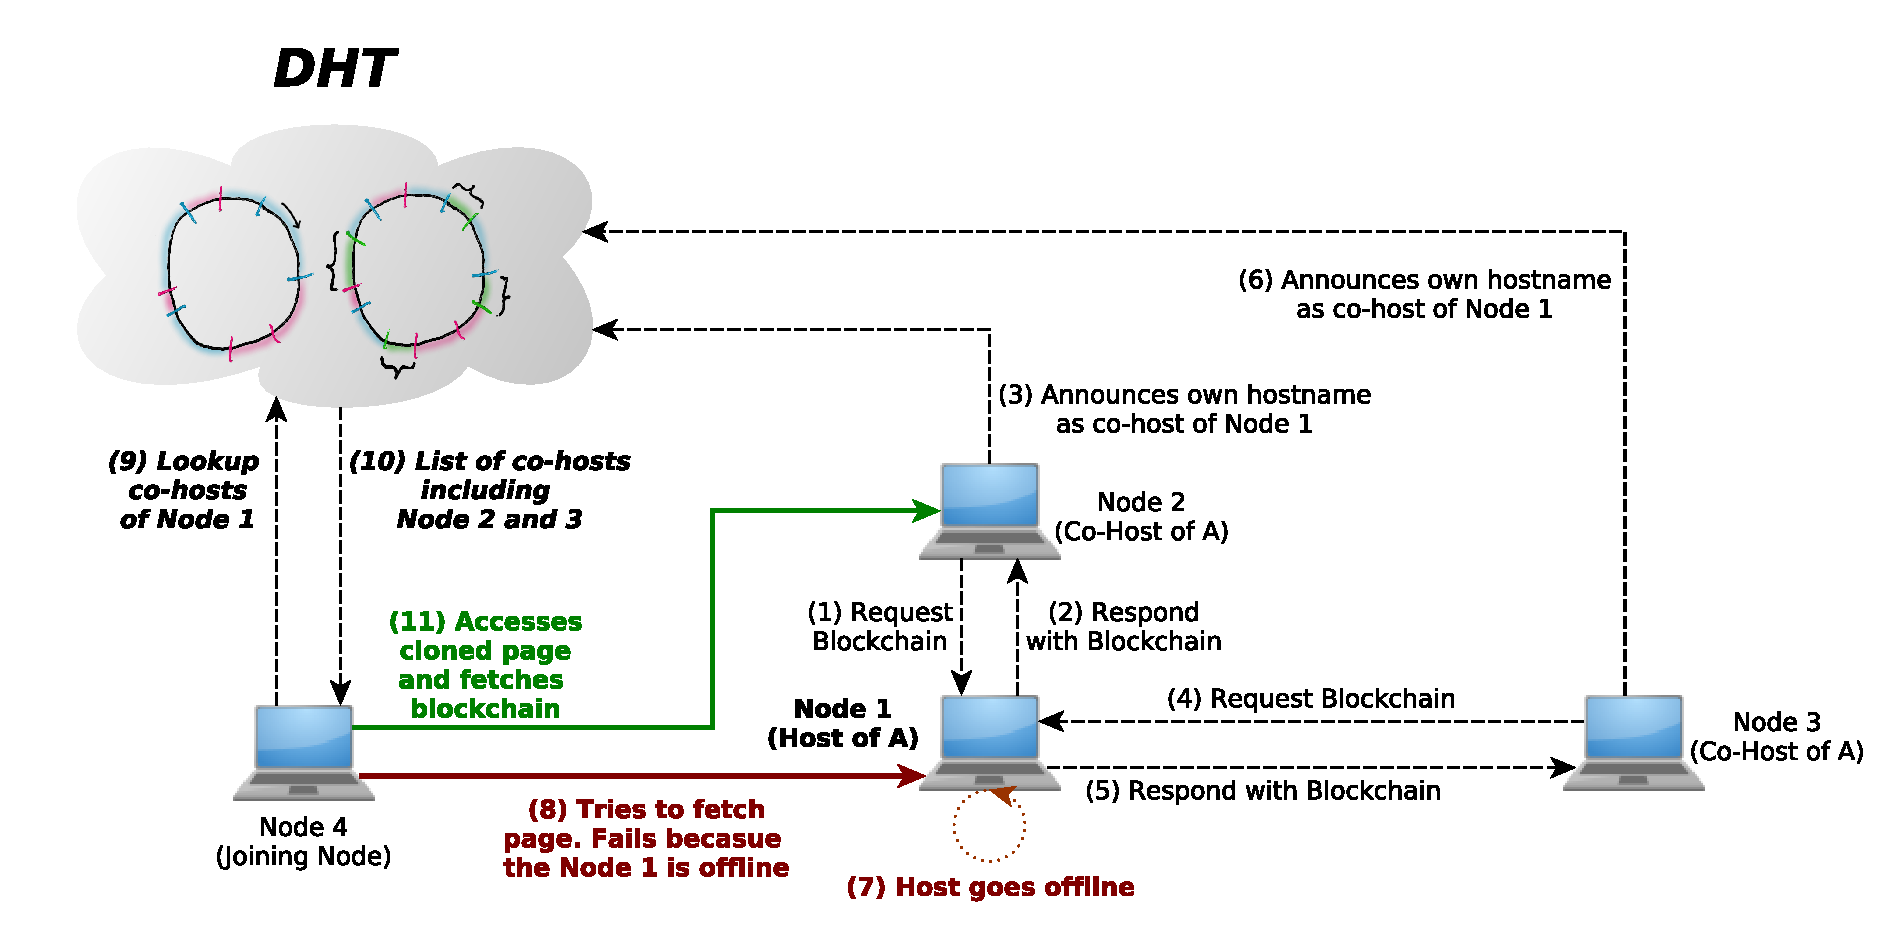
\includegraphics[width=\textwidth]{pictures/dht_solution_to_first_lookup.pdf}
\caption{Proposed solution, based on a Distributed Hash Table (DHT) for the
first lookup problem if the original host is offline.}
\label{fig:dht_solution}
\end{figure}

Figure \ref{fig:dht_solution} explains that approach. \textit{Node 1} is the
content creator and hosts a page. \textit{Node 2} and \textit{3} access the
page, fetch the blockchain and start hosting. After propagating a
\textit{CLONE} transaction to the network, they also announce themselves to
the DHT. Each time they continue hosting, e.g. coming back online,
an announce messages is send. \textit{Node 4} wants to access the page of
\textit{Node 1}, but this node is currently offline. By looking up all,
currently online co-hosts \textit{Node 4} can choose in this example between
\textit{Node 2} or \textit{3}, it chooses \textit{Node 2}.
